\documentclass[resume]{subfiles}

\begin{document}
\section{Équilibre, Stabilité, Oscillations}

\subsection{Équilibre}

En équilibre un état ne change pas. Sa dérivée est donc par conséquent nulle  

\subsubsection{Temps discret}

Si le système est homogène alors $\bar{x}=A\bar{x}$ si $\bar{x}$ est un vecteur propre A avec une valeur propre de A unité, alors tout vecteur propre $\bar{x}$ est point d'équilibre, sinon seulement l'origine est un équilibre  

Si le système est non-homogène alors $\bar{x}= A\bar{x}+b$ ou $\bar{x} = (I - A)^{-1}b$ si I n'est pas une valeur propre, alors il y a l'équilibre différent de 0

\subsubsection{Temps continu}

Si le système est homogène: $A\bar{x}=0$ Si A est non singulière, 0
est le seul équilibre, sinon il peut y en avoir d'autres  

Si le système est non-homogène à entrée constante: $A\bar{x}+b=0$ ou $\bar{x}=-A^{-1}b$ 
si A est non singulière il y a une solution unique
\begin{itemize}
\item En général, 0 est un point d'équilibre pour les systèmes à
  temps discret et continus
\item I est valeur propre critique pour les systèmes discrets, 0
  est valeur propre critique pour les systèmes continus  
\end{itemize}

\subsection{Stabilité}

Un point d'équilibre est stable si, quand il est perturbé, il tend à retourner à sa position initial, ou si au minimum il ne diverge pas.

$x(t + 1)-\bar{x} = Ax(t) + b - A\bar{x}-b$
$z(t + 1) = Az(t) z(t) = x(t) - \bar{x}$ 

On peut déterminer la stabilité du système avec ces pôles en boucles fermé.

\subsubsection{Temps discret}

\begin{figure}[H]
    \centering
    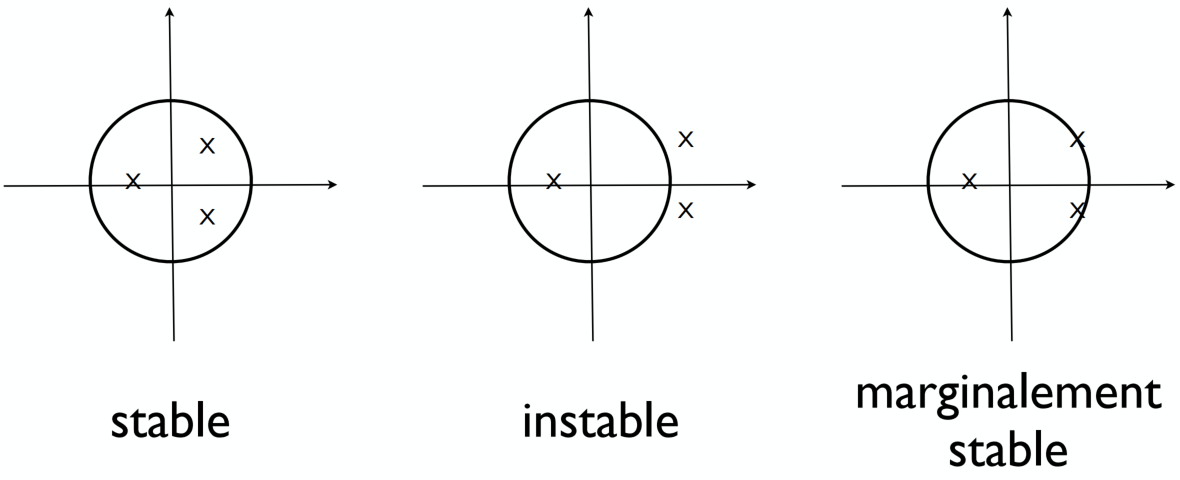
\includegraphics[width=0.8\columnwidth]{Figures/Stabilite_1.png}
\end{figure}

\subsubsection{Temps continu}

\begin{figure}[H]
    \centering
    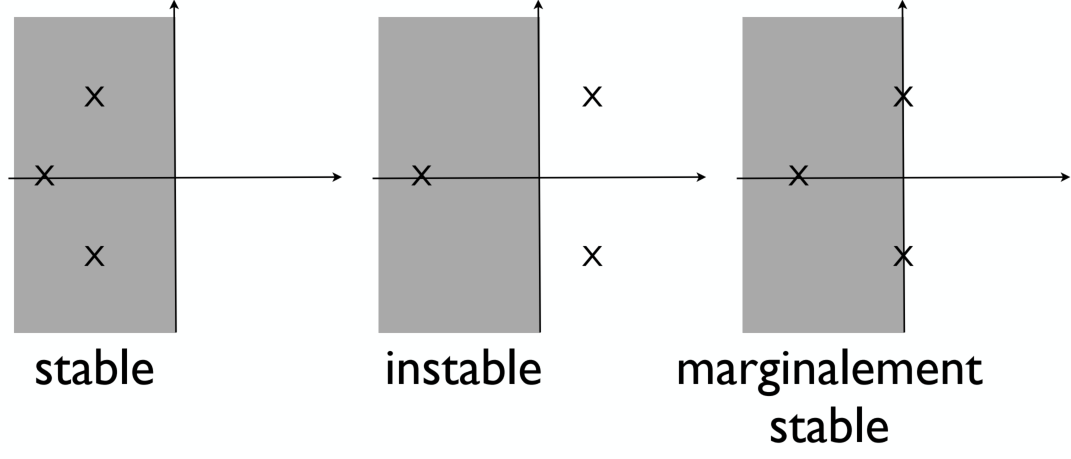
\includegraphics[width=0.8\columnwidth]{Figures/Stabilite_2.png}
\end{figure}

\subsection{Oscillations}

Les valeurs propres nous parlent de la stabilité d'un système  

Elles nous parlent également de son comportement  

Les valeurs propres peuvent s'écrire $\lambda=\mu+j\omega$ si $\omega \neq 0$ alors il y aura des oscillations

A chaque $\lambda$ il existe un $e^{\lambda}=e^{\mu}(cos(\omega t)+jsin(\omega t))$

\subsection{Pôles en boucle ouverte}
Les pôles en boucle ouverte sont les valeurs propres de $A$
\end{document}